\documentclass[pre,12pt]{revtex4-1}
\usepackage{epsfig,graphics,amssymb,amsmath,subeqnarray,setspace,graphicx,amsthm,subfigure, mathrsfs,colortbl,color,bm,fancyhdr}
\usepackage{graphicx}
\usepackage{color}

% Header on each page, with team number and page numbering
\pagestyle{fancy}
\lhead{Team \# 12345} 
\rhead{page \thepage \ of \pageref{LastPage}}
\cfoot{}
\renewcommand{\headrulewidth}{0.4pt}
\renewcommand{\footrulewidth}{0.0pt}

% Make life easier: define some shortcuts!
\def\b{\bm}
\def\e{\epsilon}
\def\ep{\varepsilon}
\def\u{\underline}
\def\c{\centerline}
\def\n{\noindent}
\def\h{\hangindent}


\newcommand{\tcb}{\textcolor{blue}}

% Double spacing is 2, 1.5 spacing is 1.5, ...
\def\baselinestretch{1.0}

% For tables:
\definecolor{Gray}{gray}{0.9}
\newcolumntype{C}{c<{\kern\tabcolsep}@{}}

\begin{document}

\title{Great Lakes Water Problem}
\author{Team \# 12345}
\date{\today}

\begin{abstract}


\end{abstract}
\maketitle

\newpage

\section{Introduction}\label{Introduction}

\section{Background}\label{Background}

\section{Assumptions}\label{Assumptions}

\section{St. Lawrence Rive, Niagara Falls, and the Water Level}\label{Model}

\begin{center}
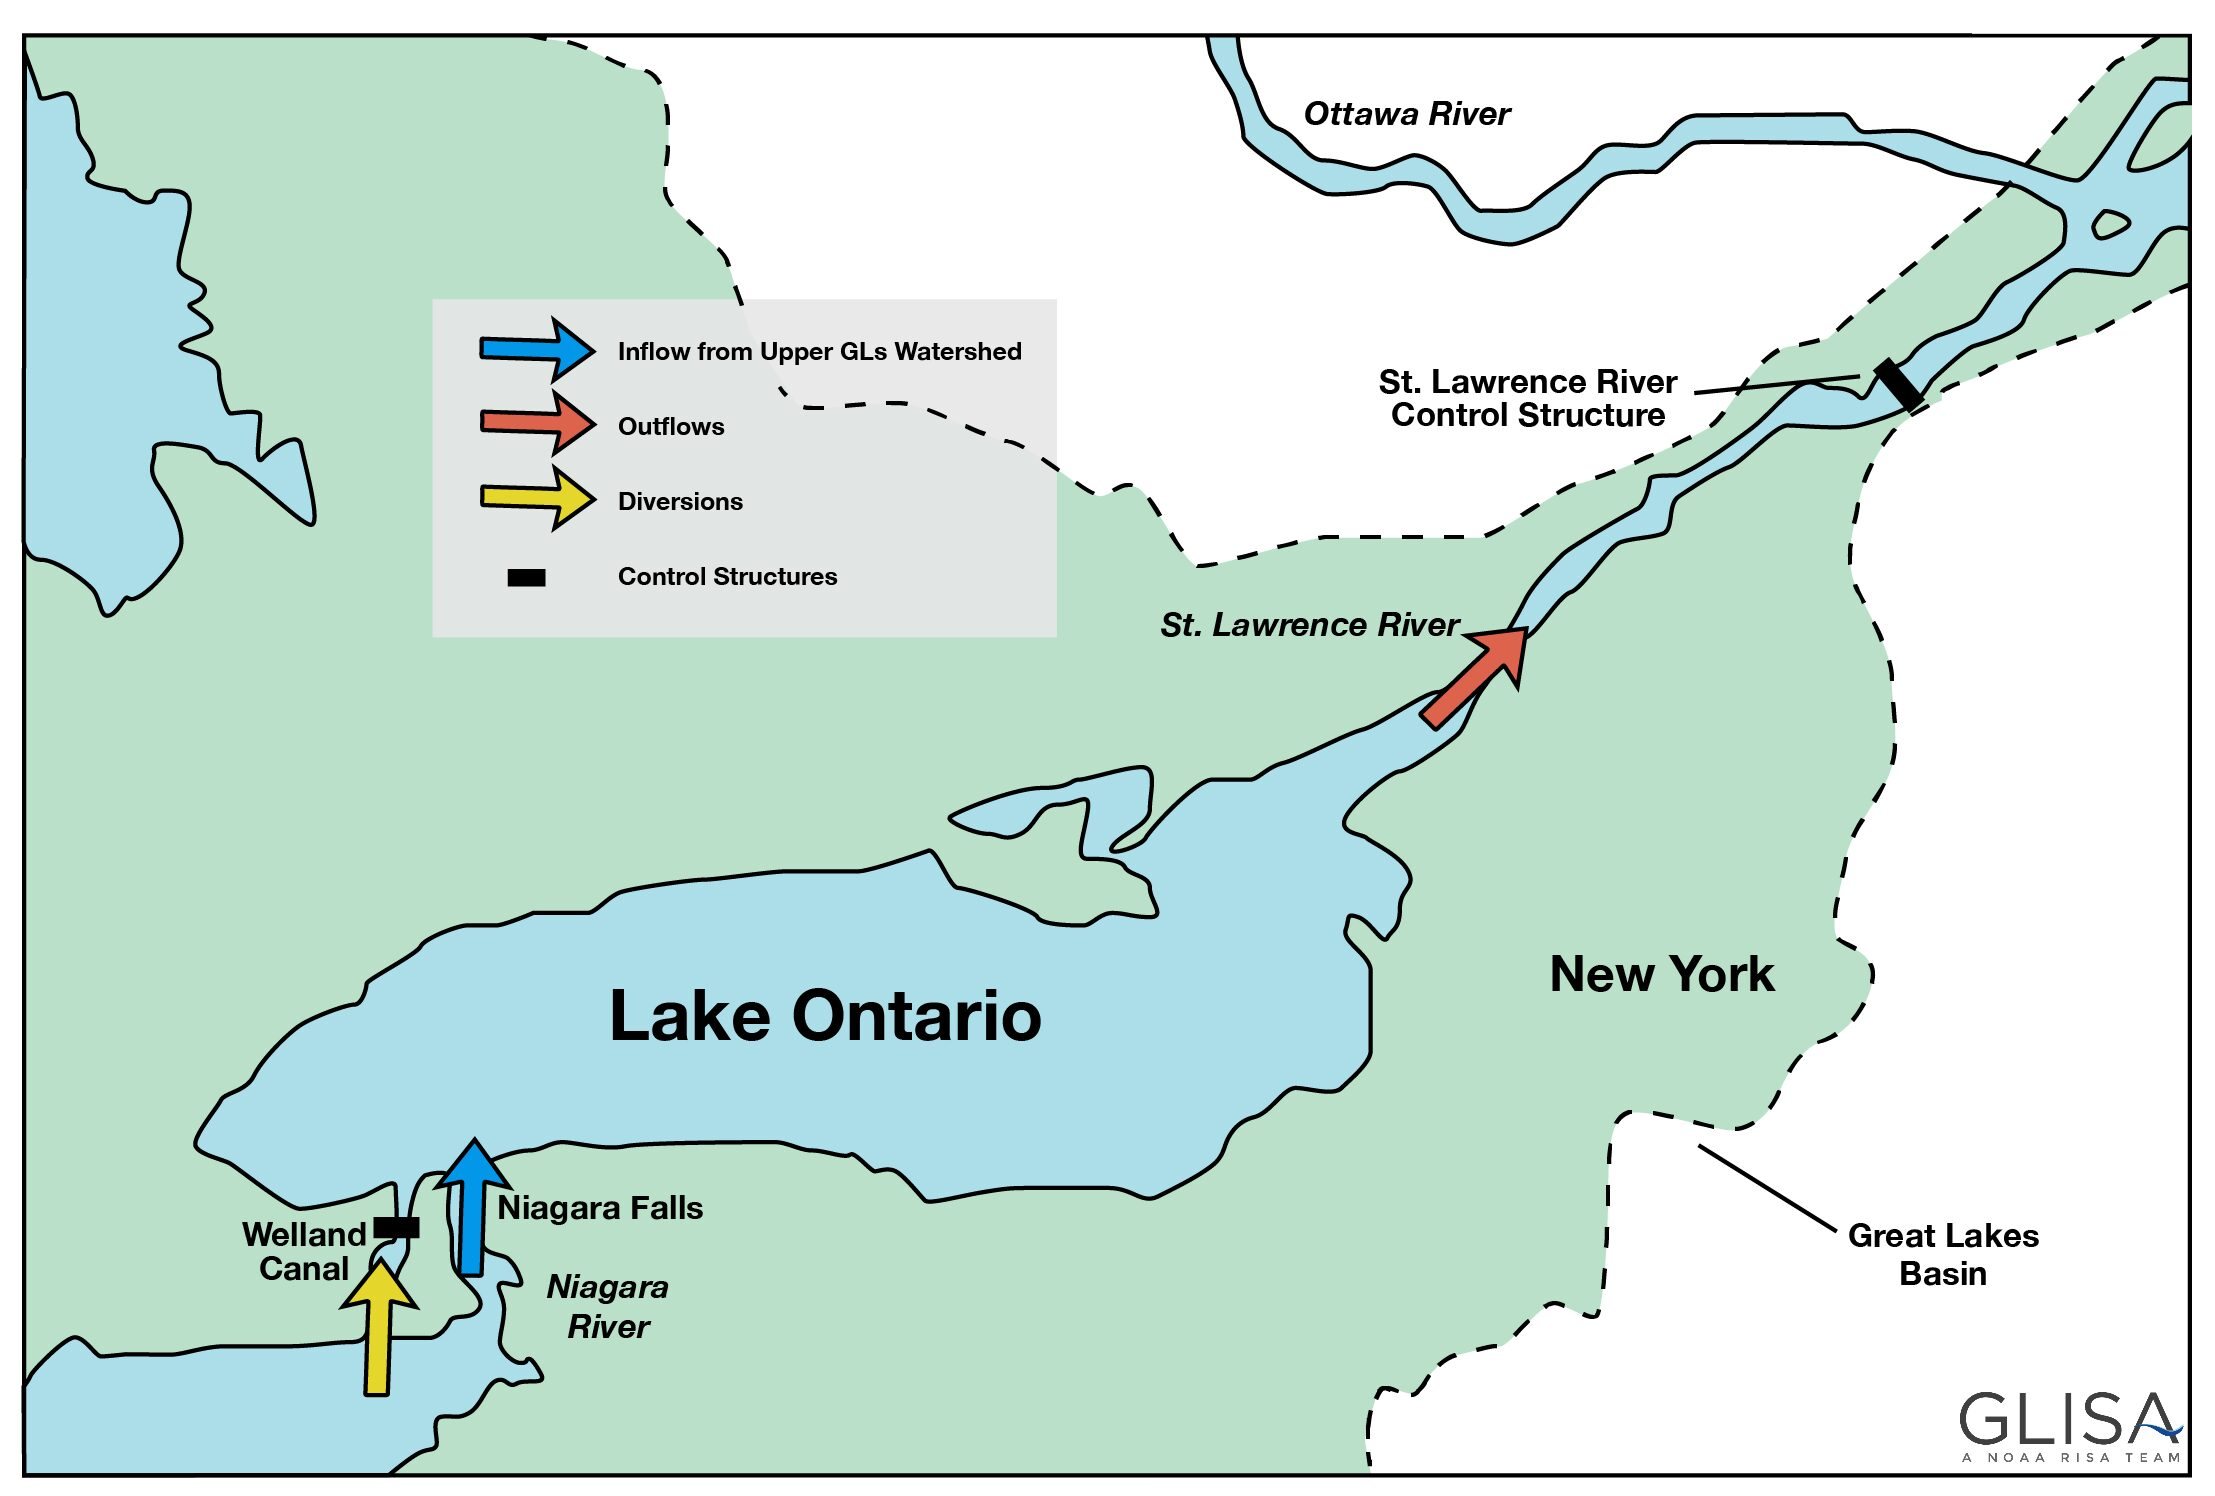
\includegraphics[width=0.75\linewidth]{img/river_flow.jpeg}
\end{center}

The Lake Ontario water level is related to the outflow of the St. Lawrence River, the inflow of the Niagara River, and the flow of the other rivers that feed into Lake Ontario. Outflow of St. Lawrence River is given by the competition. We also found the data of inflow of Niagara River, and data of the historical water level of Lake Ontario. We then used the data to analyze the pattern of the water level of Lake Ontario.

The water level of Lake Ontario appears to be related to the season. The water level seems to be higher during the summer season while lower during the winter season. 

\begin{center}
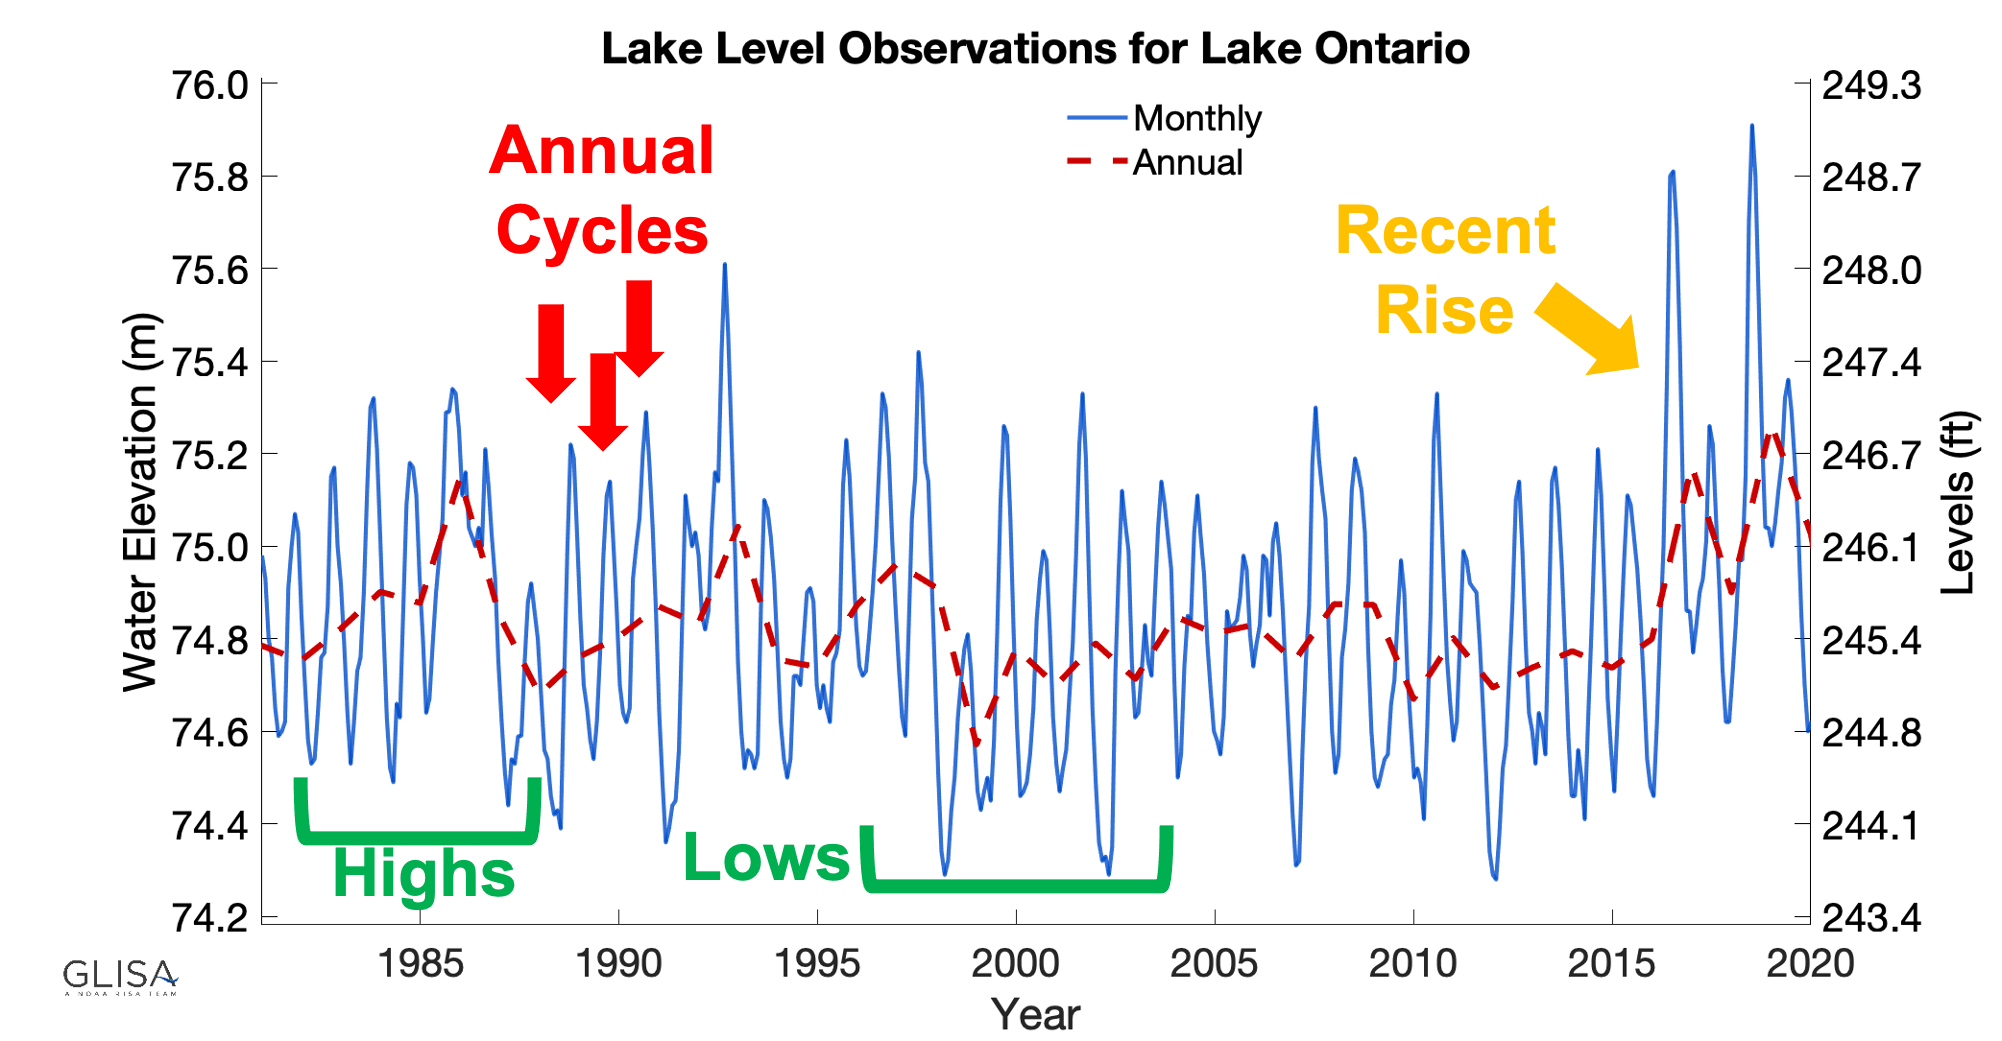
\includegraphics[width=0.8\linewidth]{img/water_level.png}
\end{center}


  After observing the periodic trends of the data. We perform Seasonal Decomposition for the two main factors that affect the water level of Lake Ontario, the outflow of St. Lawrence River and the inflow of Niagara River. We then use the seasonal decomposition to analyze the pattern of the water level of Lake Ontario. 

\subsection*{Technical formulation}

We model the water outflow as time series data, identifying underlying patterns and trends crucial for predictive modeling and environmental management. The decomposition is based on the additive model, defined by the equation \(Y_t = T_t + S_t + R_t\), where \(Y_t\) denotes the water outflow at time \(t\), \(T_t\) represents the trend component, \(S_t\) the seasonal component, and \(R_t\) the residual or irregular component.


The trend component \(T_t\) is designed to capture long-term variations in water outflow, filtering out short-term fluctuations and seasonal effects. We employ the Locally Weighted Scatterplot Smoothing (LOESS) technique for an adaptive estimation of \(T_t\), which is particularly adept at handling nonlinear trends:

\[ T_t = \sum_{i=1}^{N} w_i(t) \cdot y_i \]

where \(w_i(t)\) are weights calculated for each observation \(y_i\), based on the proximity to the point \(t\), and \(N\) is the total number of observations. These weights are typically determined using a tricubic weight function to emphasize the influence of points nearest to \(t\).


For modeling the seasonal fluctuations in river outflow, which may arise from environmental cyclical factors such as precipitation and snowmelt, the seasonal component \(S_t\) is represented as a sum of sine and cosine functions through a Fourier series. This allows for capturing complex seasonal patterns that might not adhere to strict periodicity:

\[ S_t = \alpha_0 + \sum_{n=1}^{M} [\alpha_n \cos(2\pi n f t) + \beta_n \sin(2\pi n f t)] \]

where:
\begin{itemize}
    \item \(M\) is the number of harmonics included,
    \item \(\alpha_n\) and \(\beta_n\) are the coefficients for the cosine and sine components, respectively, of the \(n\)-th harmonic,
    \item \(f\) is the fundamental frequency of the seasonal cycle, identified by the known periodicity in the data (e.g., \(f=1/12\) for monthly data reflecting an annual cycle),
    \item \(t\) represents the time index.
\end{itemize}

The coefficients \(\alpha_n\) and \(\beta_n\) are estimated via least squares regression, fitting this model to the detrended data to ensure the seasonal component closely mirrors observed cyclic patterns in water outflow.


The residual component \(R_t\) encapsulates the portion of water outflow not explained by the trend and seasonal components, reflecting irregular fluctuations due to environmental events, measurement errors, or unmodeled influences:

\[ R_t = Y_t - T_t - S_t \]

Analyzing \(R_t\) is vital for assessing the model's fit, identifying outliers, and revealing any patterns that might suggest further explanatory variables or model adjustments.


To imbue our analysis with greater mathematical depth, we explore the statistical properties of our estimated components, conducting variance analysis on \(R_t\) to ensure the residuals' homoscedasticity. Moreover, spectral analysis on \(S_t\) verifies the adequacy of our selected harmonic terms in capturing seasonal variability.

\subsection{Advanced Considerations}

\begin{itemize}
    \item \textbf{Dynamic Trend and Seasonality:} Acknowledging the dynamic nature of environmental systems, we explore model extensions allowing for time-varying trends and seasonality, applying state-space models and Kalman filtering to adjust \(T_t\) and \(S_t\) dynamically with incoming data.
    
    \item \textbf{Statistical Testing for Component Significance:} We employ the Augmented Dickey-Fuller test on \(T_t\) to assess non-stationarity, ensuring our trend component reflects true long-term movement. For \(S_t\), Fourier analysis statistically validates the significance of identified seasonal frequencies, cementing our model's foundation.
\end{itemize}

This rigorous mathematical framework enables a comprehensive understanding of river water outflow dynamics, facilitating precise forecasting and effective environmental management strategies. Through meticulous statistical and mathematical techniques, we unravel the complexities of river ecosystems, contributing to the sustainable management of water resources.


\section{Numerical method}\label{Numerics}

Describe exactly what you're going to compute, and how.

\section{Results and analysis}\label{Results}



\section{Something more}\label{Something}


\section{Discussion}\label{Discussion}

\subsection{Strengths of the model}

\subsection{Weaknesses of the model}

\subsection{Future directions}

\appendix

\section{}\label{AppendixA}


% \begin{thebibliography}{10}
% \bibitem{nd97} Nelson, Timothy, and Dengler, Nancy. ``Leaf vascular pattern formation.'' The Plant Cell 9.7 (1997): 1121.
% \end{thebibliography}
\bibliographystyle{plain}
\bibliography{references}
\end{document}

